\chapter{Für Nerds}
\label{ch:fuerNerds}
\textit{Die eigene Sammlung auf der eigenen Homepage veröffentlichen. Mit Hilfe von Plugins für OpenCms kein Problem für PUMA.}
\section{URL-Syntax\index{URL-Syntax}}
\label{sec:urlSyntax}
Sie können die Funktionen von PUMA nicht nur über das Menü (\autoref{sec:hauptmenue}) erreichen, sondern auch direkt über die URL ansteuern. Die URL ist die Adresse einer Seite, die im Adressfeld des Browsers eingegeben, bzw. angezeigt wird. Die Seite mit der Adresse \texttt{\begin{small}https://puma.ub.uni-stuttgart.de/user/mueller/forschungsdaten\end{small}} liefert beispielsweise alle Einträge des Benutzers \textit{mueller} zurück, die mit dem Tag \textit{forschungsdaten} gekennzeichnet sind.
Der Teil \texttt{https://puma.ub.uni-stuttgart.de} bezeichnet den Ort der PUMA-Installation, der Rest der URL steuert, welche Seiten oder Inhalte von PUMA zurückgegeben werden. 
 
\subsection{Allgemeine Seiten}
\label{subsec:allgemeineSeiten}
\begin{description}
    \item [/] Homepage von PUMA, zeigt die aktuellsten 50 öffentlichen Einträge.
    \item [/popular] Zeigt die 100 häufigsten Einträge der letzten 100.000 öffentlichen Einträge.
    \item [/IhrBenutzername]    Ihre persönliche Sammlung.
    \item [/help\_de]    Hilfeseite.
     \item [/myBibTeX]    Zeigt Ihre gesamte Sammlung im BibTex-Format.
    \item [/myRelations]    Zeigt Ihre Konzepte/Relationen.
    \item [/myDuplicates]    Zeigt die Duplikaten, die sich in Ihrer eigenen Sammlung befinden.
    \item [/groups]   Zeigt eine Liste aller Gruppen, die es in PUMA gibt.
    \item [/mySearch] Bietet eine Schnellsuche in Ihrer eigenen Sammlung.

\end{description}    

\subsection{Administrative Seiten}
\label{subsec:adminSeiten}
\begin{description}
\item [/settings]  Einstellungsseite. Auf dieser Seite können Sie:
    \begin{itemize}
        \item Ihr Profil bearbeiten und Kontoeinstellungen ändern,
        \item einen Benutzer zu Ihrer Gruppe hinzufügen,
        \item Ihren API-Schlüssel finden und einen neuen erzeugen,
        \item Ihr Passwort ändern und
        \item Ihre Daten zwischen BibSonomy und PUMA synchronisieren.
    \end{itemize}
    \item [/postBookmark]    Neues Lesezeichen einfügen. \hfill \\Überprüft vorab, ob sich die URL der Seite bereits in der Sammlung befindet.
    \item [/postPublication]    Neue Publikation einfügen. 
\end{description}

\subsection{Publikations- und Lesezeichenlisten nach verschiedenen Kriterien erstellen}
\label{subsec:suchenMitUrlSyntax}
PUMA bietet Ihnen die Möglichkeit mit Hilfe der URL ihre Publikationslisten nach verschiedenen Kriterien zusammenzustellen und zu filtern. Möglichke Kriterien sind: Tags, Autor, Publikationsjahr, Benutzername der Person, die den Eintrag gespeichert hat, sowie Freunde- und Gruppennamen. \newline
\newline

\subsubsection{Einträge nach Benutzer}
\label{sss:nachBenutzer}

Um die Einträge eines bestimmten Benutzers aufzulisten, verwenden Sie die Syntax \texttt{/user/<benutzername>}, wobei \texttt{<benutzername>} für den PUMA-Benutzername des gewünschten Nutzers steht. Das Ergebnis kann zusätzlich noch nach Tag gefiltert werden: \texttt{/user/<benutzername>/<tag>}. Mehrere Tags können durch ein + verknüpft werden.

Beispiele:
\begin{description}
    \item [/user/eckert] \hfill \\ 
    Zeigt alle öffentlichen Einträge des Benutzers \textit{eckert}.
    \item [/user/eckert/politik] \hfill \\
    Zeigt alle öffentlichen Einträge mit dem Tag \textit{politik} des Benutzers \textit{eckert}.
    \item [/user/eckert/politik+menschenrechte] \hfill \\
    Zeigt alle öffentlichen Einträge des Benutzers \textit {eckert} an, die sowohl mit dem Tag \textit{politik} als auch mit dem Tag \textit{menschenrechte} verschlagwortet sind.
\end{description}

\subsubsection{Einträge nach Tag\index{Tags}}
\label{sss:nachTag}
Um alle Einträge aufzulisten, die mit einem bestimmten Tag verschlagwortet sind, verwenden Sie die Syntax \texttt{/tag/<tag>}, wobei <tag> durch das gewünschte Tag ersetzt wird. Mehrere Tags können mit einem + verknüpft werden.

Beispiele:
\begin{description}
    \item [/tag/politik] \hfill \\
    Zeigt alle öffentlichen Einträge mit dem Tag \textit{politik} an.
    \item [/tag/politik+menschenrechte] \hfill \\
    Zeigt alle öffentlichen Einträge an, die sowohl mit dem Tag \textit{politik} als auch mit dem Tag \textit{menschenrechte} verschlagwortet sind.
\end{description}

\subsubsection{Einträge nach Autor\index{Autoren}}
\label{sss:nachAutor}

Um alle Publikationen eines bestimmten Autors aufzulisten, verwenden Sie die Syntax \texttt{/autor/<name>}, wobei <name> durch den Nachnamen des Autors ersetzt wird. Die Liste lässt sich mit Hilfe der Syntax \texttt{/autor/<name>/<tag>} auf bestimmte Tags eingrenzen oder durch \texttt{/autor/<name>/sys:<systemtag>:<wert>} mit verschiedenen Systemtags (siehe auch \autoref{sss:systemtags}) weiter einschränken.

Beispiele:
\begin{description}
    \item [/author/müller] \hfill \\
    Zeigt alle Publikationen des Autors mit dem Namen \textit{Müller} an.
    \item [/author/müller/dblp] \hfill \\
    Zeigt alle Einträge des Autors \textit{Müller} an, die mit dem Tag \textit{dblp} versch
    \item [/author/müller/sys:user:eckert] \hfill \\
    Zeigt alle Publikationen des Autors \textit{Müller} in der Sammlung von \textit{Eckert} an.
    \item [/author/müller/sys:group:puma] \hfill \\
    Zeigt alle Publikationen des Autors \textit{Müller} in der Sammlung aller Gruppenmitglieder der Gruppe \textit{puma} an. 
\end{description}

Mit dem Systemtag \textit{year} lässt sich das Ergebnis auf ein bestimmtes Erscheinungsjahr oder einen bestimmten Zeitraum beschränken:%muss rausrücken

Beispiele:
\begin{description}
    \item [/author/hotho/sys:year:2007] \hfill \\
    Zeigt alle Publikationen des Autors \textit{Hotho} aus dem Jahre 2007.
    \item [/author/hotho/sys:year:2003-2007] \hfill \\
    Zeigt alle Publikationen des Autors \textit{Hotho} zwischen 2003 und 2007.
    \item [/author/hotho/sys:year:-2005] \hfill \\
    Zeigt alle Publikationen des Autors \textit{Hotho} bis zum Jahr 2005 an.
    \item [/author/hotho+sys:year:1997-] \hfill \\
    Zeigt alle Publikationen des Autors \textit{Hotho} seit 1997 an.
\end{description}

\subsubsection{Einträge von Freunden} 
\label{sss:vonFreunden}
Um die Einträge Ihrer Freunde (\autoref{sec:freunde}) zu sehen, verwenden Sie die Syntax \texttt{/friends}, für alle Freunde oder \texttt{/friend/<name>} für die Einträge eines bestimmten Freundes. Sie können die Ergebnisse wie gewohnt durch die Angabe von Tags weiter einschränken. 

Sie sehen nur die Einträge, die von Benutzern stammen, auf deren Freundesliste Sie stehen und die von diesen Benutzern für Freunde freigegeben wurden (für Freunde sichtbar).

Beispiele:
\begin{description}
    \item [/friends] \hfill \\
    Zeigt die für Freunde gekennzeichneten Einträge aller ihrer Freunde.
    \item [/friend/eckert] \hfill \\
    Zeigt die für Freunde gekennzeichneten Einträge des Benutzers \textit{eckert}. Sie können diese Einträge nur dann sehen, wenn \textit{eckert} Sie als Freund angegeben hat.
    \item [/friend/eckert/politik] \hfill \\
    Zeit die für Freunde gekennzeichneten Einträge des Benutzers \textit{eckert} an, die mit dem Tag \textit{politik} verschlagwortet wurden. 
    \item [/friend/eckert/politik+menschenrechte] \hfill \\
    Zeigt die für Freunde gekennzeichneten Einträge des Benutzers \textit{eckert} an, die sowohl mit dem Tag \textit{politik} als auch mit dem Tag \textit{menschenrechte} verschlagwortet sind. 
\end{description}

\subsubsection{Einträge nach Sichtbarkeit}
\label{sss:nachSichtbarkeit}
Um zu sehen, welche ihrer Einträge für wen sichtbar sind, können Sie die Syntax \texttt{/viewable/<sichtbarkeit>} verwenden. Als \texttt{<sichtbarkeit>} sind folgende Ausprägungen möglich:
\begin{description}
  \item[public] Einträge, die öffentlich sichtbar sind
	\item[private] Einträge, die nur für Sie selber sichtbar sind
	\item[friends] Einträge, die für die Benutzer sichtbar sind, die auf ihrer Freundeliste stehen
	\item[<gruppenname>] Einträge, die für die Mitglieder der Gruppe <gruppenname> sichtbar sind
\end{description}  

Die Ergebnisse können mit Hilfe der Syntax \texttt{/viewable/<sichtbarkeit>/<tags>} zusätzlich durch Tags eingeschränkt werden. 

Beispiele:
\begin{description}
    \item [/viewable/public] \hfill \\
    Zeigt alle Ihre Einträge an, die Sie als \enquote{öffentlich sichtbar\index{Sichtbarkeit!öffentlich}} eingestellt haben.
    \item [/viewable/public/politik] \hfill \\
    Zeigt alle Ihre öffentlich sichtbaren Einträge, die mit dem Tag \textit{politik} verschlagwortet wurden.
    \item [/viewable/private] \hfill \\
    Zeigt alle Ihre Einträge, die Sie als \enquote{privat sichtbar\index{Sichtbarkeit!privat}} eingestellt haben.
    \item [/viewable/private/politik+menschenrechte] \hfill \\
    Zeigt alle Ihre Einträge an, die nur für Sie sichtbar sind und sowohl mit dem Tag \textit{politik} als auch mit dem Tag \textit{menschenrechte} verschlagwortet wurden. 
    \item [/viewable/friends] \hfill \\
    Zeigt alle Ihre Einträge an, die Sie als \enquote{für Freunde sichtbar\index{Sichtbarkeit!Freunde}} eingestellt haben.
    \item [/viewable/puma] \hfill \\
    Zeigt alle Einträge an, die für die Gruppe \textit{puma} als sichtbar eingestellt wurden.
    \item [/viewable/puma/politik] \hfill \\
    Zeigt alle Einträge an, die für die Gruppe \textit{puma} sichtbar sind und mit dem Tag \textit{politik} verschlagwortet wurden.
\end{description}

\subsubsection{Einträge nach Gruppe\index{Gruppen}}
\label{sss:nachGruppe}
Wenn Sie Mitglied einer Gruppe (\autoref{sec:gruppen}) sind, können Sie mit Hilfe der Syntax \texttt{/group/<gruppenname>} die Einträge aller Gruppenmitglieder auflisten. Die Ergebnisse können mit \texttt{/group/<gruppenname>/<tags>} nach Tags gefiltert werden.

Beispiele:
\begin{description}
    \item [/group/puma] \hfill \\
    Zeigt Ihnen alle Einträge von Mitgliedern der Gruppe \textit{puma} an, wenn Sie Gruppenmitglied sind.
    \item [/group/puma/politik] \hfill \\
    Zeigt Ihnen alle Einträge von Mitgliedern der Gruppe \textit{puma} an, die mit dem Tag \textit{politik} verschlagwortet sind. 
    \item [/group/puma/politik+menschenrechte] \hfill \\
    Zeigt Ihnen alle Einträge von Mitgliedern der Gruppe \textit{puma} an, die mit dem Tag \textit{politik} und dem Tag \textit{menschenrechte} verschlagwortet sind. 
    \item [/relevantfor/group/puma] \hfill \\
    Zeigt Ihnen alle Einträge an, die ein Gruppenmitglied der Gruppe \textit{puma} als relevant für diese Gruppe gekennzeichnet hat.
    \item [/followers] \hfill \\
    Zeigt die neuesten Einträge aller Benutzer, denen Sie folgen. Diese Einträge werden mittels eines Rankings so umsortiert, dass die für Sie relevantesten Einträge ganz oben stehen. 
\end{description}



\paragraph*{Umgang mit Duplikaten\index{Duplikate}}
\label{subsec:duplikate}
Wenn innerhalb einer Gruppe zwei oder mehr Benutzer denselben Eintrag in ihrer Sammlung haben, kommt es vor, dass Einträge (Publikationen) mehrfach auf einer Gruppenseite angezeigt werden. Falls dies nicht gewünscht ist, kann das Verhalten mittels des Parameters \textit{duplicates} angepasst werden. Der Parameter kann folgende Ausprägungen haben:
\begin{description}
\item [yes] Jeder Eintrag wird angezeigt, auch wenn er ein Duplikat darstellt (Standard).
  \item[no] Bei Duplikaten wird jeweils nur der erste Eintrag angezeigt.
  \item [merged] Die Tags aller Duplikate werden gesammelt an einem einzelnen Eintrag angezeigt.
  \end{description}

Beispiele:
\begin{description}
    \item [/group/puma?duplicates=no] \hfill \\
    Zeigt alle Einträge der Gruppe \textit{puma} an. Für jedes Duplikat wird nur der erste Eintrag angezeigt.
    \item [/group/puma?duplicates=merged] \hfill \\
    Zeigt alle Einträge der Gruppe \textit{puma} an. Für jedes Duplikat werden alle Tags \enquote{aufgesammelt} und aggregiert an einem einzelnen Eintrag angezeigt.
\end{description}

\subsubsection{Weitere Filterkriterien}
\label{sss:weitereKriterien}

PUMA bietet noch weitere Kriterien, nach denen Ergebnislisten zusammengestellt und gefiltert werden können. Mit der Syntax \texttt{/url/<hashkey>} werden alle Lesezeichen angezeigt, deren URL den Hash <hashkey> haben. Veröffentlichnungen mit einem bestimmten Intra-Hash (siehe \autoref{sec:duplikat}) erreichen Sie mit der Syntax \texttt{/bibtex/<intrahas>}. Mit der Syntax \texttt{/bibtexkey/<bibtexkey>} können Sie Veröffentlichungen mit einem bestimmten BibTeX-Key anzeigen.



\subsection{Konzeptseiten}
\label{subsec:konzeptseiten}
Konzepte (\autoref{subsec:konzepte}) sind Überbegriffe, mit denen Sie Ihre Tags strukturiert können. Um die Konzepte eines Benutzers anzuzeigen, verwenden Sie die Syntax \texttt{/concepts/<benutzername>}. Um die Lesezeichen oder Publikationen zu erhalten, die mit einem Konzept oder eines seiner Untertags verschlagwortet wurden, verwenden Sie die Syntax \texttt{/concept/user/<benutzername>/<konzept>}.

Beispiele:
\begin{description}
    \item [/concepts/eckert] \hfill \\
    Zeigt alle Konzepte\index{Konzepte} des Benutzers \textit{eckert} angezeigt.
    \item [/concept/user/eckert/psychologie] \hfill \\
    Zeigt alle Lesezeichen und Publikationen des Benutzers \textit{eckert} an, denen das Konzept \textit{psychologie} oder eines seiner Unterschlagwörter als Tag zugeordnet ist. 
\end{description}

\subsection{Volltextsuche}
\label{subsec:volltext}
Die Volltextsuche von PUMA wird über die URL-Syntax \texttt{/search/<suchbegriff>} gesteuert. Mehrere Suchbegriffe können mit einem \texttt{+} verknüpft werden. Ein \texttt{-} vor einem Suchbegriff bewirkt, dass nur Einträge zurückgeliefert werden, die den entsprechenden Suchbegriff \textbf{nicht} enthalten. Ein Suchbegriff kann mit der Syntax \texttt{user:<benutzername>} auch den Benutzer festlegen, in dessen Einträgen gesucht werden soll.

Die Volltextsuche sucht in den Feldern Titel und Beschreibung (bei Lesezeichen auch noch in der URL) nach allen Einträgen, die den Suchbegriff oder die Suchbegriffe enthalten.

Beispiele:
\label{subsec:volltextsuche}
\begin{description}
    \item [/search/politik] \hfill \\
    Zeigt alle öffentlichen Einträge an, die das Wort \textit{politik} enthalten. 
    \item [/search/politik+menschenrechte] \hfill \\
    Zeigt alle öffentlichen Einträge, die das Wort \textit{politik} und das Wort \textit{menschenrechte} enthalten. 
    \item [/search/politik+-menschenrechte] \hfill \\
    Zeigt alle öffentlichen Einträge, die das Wort \textit{politik}, aber nicht das Wort \textit{menschenrechte} enthalten. 
    \item [/search/politik+user:droessler] \hfill \\
    Zeigt alle öffentlichen Einträge des Benutzers \textit{droessler}, die das Wort \textit{politik} enthalten. 
    \item [/search/politik+menschenrechte+user:droessler] \hfill \\
    Zeigt alle öffentlichen Einträge des Benutzers \textit{droessler} an, die das Wort \textit{politik} und das Wort \textit{menschenrechte} enthalten. 
    \item [/search/politik+-menschenrechte+user:droessler] \hfill \\
    Zeigt alle öffentlichen Einträge des Benutzers \textit{droessler} an, die das Wort \textit{politik}, aber nicht das Wort \textit{menschnerechte} enthalten. 
\end{description}


\subsection{Export von Einträgen}
\label{export}
PUMA bietet Ihnen die Möglichkeit, Ihre Lesezeichen und Publikationen in viele verschiedene Formate zu exportieren.
Die Exportfunktion von PUMA steuern Sie mit der Syntax \texttt{/<exportformat>}. Als Exportformat können Sie aus den folgenden Möglichkeiten wählen.

\begin{itemize}
    \item RSS Feeds\index{RSS}
    \begin{description}
        \item [/publrss/] Liefert einen RSS-Feed zurück.
        \item [/burst/]  Liefert einen BuRST-Feed zurück.
        \item [/aparss/] Liefert einen RSS-Feed im APA-Format zurück.
    \end{description}
    \item Strukturierte Daten
    \begin{description}
        \item [/bib/] Gibt die Einträge im BibTeX-Format\index{BibTex} zurück.
        \item [/endnote/] Gibt die Einträge im EndNote-Format\index{EndNote} zurück.
        \item[/json/] Gibt die Einträge im JSON-Format zurück.
        \item[/swrc/] Gibt die Einträge im  RDF-Format gemäß der SWRC-Ontologie für das Semantic Web zurück.
    \end{description}
    \item HTML\index{HTML}
    \begin{description}
        \item [/publ/] Gibt die Einträge als HTML-Tabelle zurück.
        \item [/publ/?notags=1] Gibt die Einträge ohne Tags als HTML-Tabelle zurück.
    \end{description}
  \item JabRef-Layouts
    \begin{description}
  \item[/layout/simplehtml/] Gibt die Einträge im HTML-Format als einfache Auflistung zurück.
  \item[/layout/html/] Gibt die Einträge im HTML-Format als formatierte Aufzählung zurück.
  \item[/layout/tablerefs/] Gibt die Einträge im HTML-Format als durchsuchbare Tabelle zurück.
  \item[/layout/tablerefsabsbib/] Gibt die Einträge im HTML-Format als durchsuchbare Tabelle zusätzlich mit aufklappbarem Abstract und BibTeX-Eintrag zurück.
  \item[/layout/docbook/] Gibt eine XML-Datei im Docbook-Format zurück.
  \item[/layout/dblp/] Gibt eine XML-Datei im DBLP-Format zurück.
  \item[/layout/endnote/] Gibt eine Text-Datei zurück, die vom Literaturverwaltungsprogramm EndNote verarbeitet werden kann
  \item[/layout/text/] Gibt eine Text-Datei im BibTeX-Format zurück.
    \end{description}
\end{itemize}

Die zu exportierenden Einträge können Sie dann über die Syntax \texttt{/<exportformat>/user/<benutzername>/<tags>} nach Benutzer filtern und auch zusätzlich noch auf bestimmte Tags einschränken. Möchten Sie nur nach Tag und nicht nach Benutzer filtern, verwenden Sie die Syntax \texttt{/<exportformat>/tag/<tags>}. Analog können Sie auch die anderen Kriterien zur Filterung der Ausgabe verwenden die im \autoref{subsec:suchenMitUrlSyntax} beschrieben sind.

Beispiele:
\label{subsec:volltextsuche}
\begin{description}
    \item [/bib/user/droessler] \hfill \\
    Gibt alle Einträge des Benutzers \textit{droessler} im BibTeX-Format aus.
    \item [/publrss/group/testgroup] \hfill \\
      Liedert einen RSS-Feed zurück, der die Einträge der Gruppe \textit{testgroup} enthält.
    \item [/layout/tablerefs/tag/fdm] \hfill \\
      Gibt eine durchsuchbare Tabelle im HTML-Format zurück, die alle Einträge mit dem Tag \textit{fdm} enthält. 
\end{description}

%nach hinten verschieben
\subsection{Parameter}
\label{subsec:parameter}
Mit einem Fragezeichen können an eine URL noch Parameter angehängt werden, die die Ausgabe steuern (Sortierung, Anzahl angezeigter Einträge). Mehrere Parameter werden durch ein \& getrennt. Die URL \texttt{\begin{small} /user/mueller?items=25\&sortPage=author\&sortPageOrder=desc\end{small}} liefert zum Beispiel die ersten 25 Einträge des Benutzers \textit{mueller} sortiert absteigend nach dem Autor. 

Immer wenn Sie in PUMA eine Liste von Lesezeichen oder Publikationen ausgeben, können Sie diese sortieren, indem Sie an die URL einen oder mehrere der folgenden Suchparameter anhängen. Folgende Parameter stehen Ihnen zur Verfügung:
\begin{description}
    \item [sortPage] Wonach wird sortiert?
    \begin{description}
        \item [author] Autorenname
        \item [editor] Herausgebername
        \item [year] Erscheinungsjahr
        \item [entrytype] Publikationstyp
        \item [title] Titel
        \item [booktitle] Buchtitel (insb. bei Artikel in Sammelbänden)
        \item [journal] Journalname
        \item [school] Universitätsname 
    \end{description}
    \item [sortPageOrder] Reihenfolge der Sortierung
    \begin{description}
        \item [asc] aufsteigend
        \item [desc] absteigend 
    \end{description}
\end{description}

Die Parameter \texttt{items} und \texttt{duplicates} steuern wieviele Einträge mit oder ohne Duplikate angezeigt werden:

\begin{description}		
    \item [items] Wieviele Einträge werden angezeigt\hfill \\
		 Wenn dieser Parameter nicht angegeben ist, werden standardmäßig 20 Einträge angezeigt.
    \item [duplicates] Duplikate\index{Duplikate}
    \begin{description}
        \item [yes] Erlaubt Duplikate in der Lesezeichen/- Publikationsliste
        \item [no] Entfernt Duplikate aus der Ergebnisliste
    \end{description}
\end{description}
%Beispiel: \url{?sortPage=year%\&sortPageOrder=asc\&duplicates=no} \newline
%Beispielkasten einfuegen
%Sortiere nach Erscheinungsjahr (sortPage=~year) aufsteigend (sortPageOrder=~asc) und entferne alle Duplikate (duplicates=~no). \newline


\section{Duplikatserkennung\index{Duplikat}} 
\label{sec:duplikat}
Die Duplikatserkennung von PUMA basiert auf Hashkeys. PUMA berechnet für jede Publikation zwei Hash Keys, den intrahash (zur Duplikatserkennung innerhalb der Sammlung eines Benutzers) und den interhash (zur Duplikatserkannung zwischen den Sammlungen verschiedener Benutzer). Zur Berechnung der Keys werden Titel, Autor und Jahr (beim intrahash zusätzlich noch Typ, Zeitschriften- oder Buchtitel, Band und Nummer) aneinander gefügt und ein Hash-Wert über dieser Zeichenfolge berechnet. Wird nun eine Publikation zum zweiten Mal in die Sammlung eingetragen, vergibt PUMA an diese Publikation den gleichen, schon vorhandenen Hashkey. Das System bemerkt die doppelte Vergabe und kennzeichnet die Publikationseinträge als Duplikate. 


\section{REST-API\index{REST-API}}
\label{sec:restApi}
PUMA bietet einen Webservice auf REST-Basis (Representational State Transfer) an. REST-Schnittstellen basieren auf dem HTTP-Protokoll und bedienen sich der Befehle GET (Informationen abrufen), POST (neue Einträge anlegen), PUT (bestehende Einträge aktualisieren) und DELETE (Einträge löschen). Die REST-Schnittstelle von PUMA dient dazu, anderen Programmen oder Skripten Zugriff auf die Daten und Funktionalitäten von PUMA zu geben. Damit wird eine automatisierte Verarbeitung der in PUMA gespeicherten Sammlungen möglich.

\subsection{API-Clients für verschiedene Programmiersprachen}
\label{subsec:apiClients}
Um die Ansprache der API zu erleichtert, gibt es für verschiedene Programmiersprachen Pakete oder Bibliotheken, die bereits einen Client implementiert haben, der die Kommunikation mit der REST-API regelt.

\begin{description}
\item [Java] \hfill \\
  Der bibsonomy-rest-client \footnote{\url{https://bitbucket.org/bibsonomy/bibsonomy/src/tip/bibsonomy-rest-client/}} ist ein Java-Modul, das einen das die Kommunikation mit der REST-API von PUMA erleichtert. Zur API gibt es eine ausführliche Dokumentation mit Beispielen\footnote{\url{https://bitbucket.org/bibsonomy/bibsonomy/wiki/documentation/api/Java\%20API\%20Examples}}. Als PUMA-Nutzer muss die URL (endpoint) auf https://puma.ub.uni-stuttgart.de/ gesetzt werden.
\item [PHP] \hfill \\
  Die restclientp-php Bibliothek\footnote{\url{https://bitbucket.org/bibsonomy/restclient-php/}} bietet einen API-Client für PUMA und Bibsonomy. 
\item [Python] \hfill \\
 Für Python gibt es eine Bibsonomy-Klasse\footnote{\url{https://bitbucket.org/bibsonomy/bibsonomy-python/]}, die die Anfragen auf die REST-Schnittstelle implementiert. 
  \end{description}

\subsection{Authentifizierung zum Zugriff auf die API}
\label{subsec:apiAuth}

Um per API-Schnittstelle auf Ihre Inhalte in PUMA zugreifen zu können, müssen Sie sich gegenüber PUMA authentifizieren. Das geht entweder mit einem individuellen API-Key oder über das Protokoll OAuth.

\subsubsection{Authentifizierung per API-Key}
\label{sss:apiKey}

Ihren individuellen API-Key finden Sie in den Einstellungen (\autoref{sec:einstellungen}) im Reiter \textit{Einstellungen} unter \textit{API}. An dieser Stelle haben Sie auch die Möglichkeit, einen neuen Key zu erzeugen. Diesen Key übergeben Sie beim Aufruf der Schnittstelle als \textit{USERNAME}. 


\subsubsection{Authentifizierung über OAuth}
\label{sss:oAuth}
OAuth\index{OAuth} ist ein etabliertes Protokoll für sichere API-Authorisierung, die es Ihnen ermöglicht, einer weiteren Anwendung den Zugriff auf ihre Daten zu erlauben. Hierfür müssen sie einen OAuth Consumer Key sowie ein Consumer Secret beantragen. Wie Sie dabei genau vorgehen erfahren Sie in der Onlinehilfe von PUMA.\footnote{\url{https://puma.ub.uni-stuttgart.de/help_de/OAuth}}

%bis hier überarbeitet


\section{Eigenen Webseiten}
\label{sec:eigeneWebseiten}
Es gibt mehrere Möglichkeiten, Inhalte aus PUMA oder Links zu PUMA auf Ihrer eigenen Webseite zu integrieren.

\subsection{Bookmarklinks\index{Bookmarklinks}}
\label{subsec:bookmarklinks}
Einige Webseiten bieten  auf Ihrer Seite einen Bookmarklink an, damit der Benutzer ganz einfach Artikel der Seite in sozialen Netzwerken teilen oder in einem Lesezeichensystem speichern kann. 
\newline Auch PUMA verfügt über einen Bookmarklink, den Sie auf Ihrer eigenen Webseite oder Blog hinzufügen können. Fügen Sie dafür einen kurzen JavaScript-Code\index{JavaScript-Code} ein (dieser befindet sich auf der \enquote{Browser Add-ons \& Bookmarklets Seite}\footnote{\url{https://puma.ub.uni-stuttgart.de/buttons}}) und schon können Ihre Besucher zu Ihren Publikationen und Lesezeichen bei PUMA gelangen.

\subsection{Publikationslisten\index{Publikationslisten}}
\label{subsec:publikationslisten}
Integrieren Sie Publikationslisten\index{Publikationslisten!Eigene Publikationslisten} (z.~B. Ihre eigenen Publikationen), die das gleiche Format haben wie in PUMA, auf Ihrer Webseite. Dazu müssen Sie ein iframe in Ihren HTML-Code\index{HTML} einfügen, das folgendermaßen aussieht:\newline %Screenshot
Die URL kann jede beliebige Seite aus PUMA sein, z.B. Ihre Benutzerseite oder die Seite einer Ihrer Gruppen. 
\begin{figure}[h!]
 \centering
 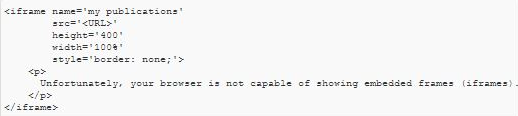
\includegraphics[width=9cm]{Bilder/Kapitel9/HTML-Code.PNG}
 \caption{HTML-Code}
 \label{fig:htmlCode}
\end{figure}
\begin{mdframed}[style=mdfexample1,frametitle={WICHTIG},backgroundcolor=gray!40]Am Ende der URL muss der Parameter \textit{format=embed} steht. Beispielsweise zeigt die URL \url{https://puma.ub.uni-stuttgart.de/user/droessler/myown?items=1000&resourcetype=publication&sortPage=year&sortPageOrder=desc&format=embed}
 alle (bis zu 1000) Publikationen des Nutzers \textit{droessler} an, denen das Schlagwort \enquote{myown} zugeordnet wurde, absteigend nach Jahr sortiert.
\end{mdframed}
\subsection{JSON-Feed\index{JSON-Feed}}
\label{subsec:jsonFeed}
Sie können für jede PUMA-Seite einen JSON-Feed\footnote{\url{http://www.json.org/}} generieren, indem Sie \textit{json/} vor den Pfadteil der URL stellen. Um beispielsweise den JSON-Feed für \textit{/tag/json} zu bekommen, geben Sie \textit{/json/tag/json} ein.

Sie erhalten einen JSON-Feed, der mit Exhibit\footnote{\url{http://www.simile-widgets.org/exhibit/}} kompatibel ist und alle Lesezeichen und Publikationen der entsprechenden Seite enthält. Um den JSON-Feed in Ihr Exhibit einzugeben, fügen Sie einen Link dazu in den Header Ihres Exhibit HTML Codes:\newline
\newline
<link href="https://puma.ub.uni-stuttgart.de/tag/json?callback=cb" type=\enquote{application/jsonp} rel=\enquote{exhibit/data} ex:jsonp-callback=\enquote{cb}%muss noch geschaut werden wegen den " 
\newline
%  Ist von kassel :  Schauen Sie sich diese Liste von Publikationen\footnote{\url{http://www.kde.cs.uni-kassel.de/hotho/publication_json.html}} an, um zu sehen, welche Möglichkeiten Sie mit JSON und Exhibit haben.

\subsection{Zope\index{Zope}}
\label{subsec:zope}
Sie können Inhalte aus PUMA dem Content Management System von Zope\footnote{\url{http://www.zope.org/}} hinzufügen.
\begin{enumerate}
    \item Publikationen\newline
    Publikationslisten können mit Hilfe des PUMA-RSS-Feeds\index{RSS} auf Ihrer Zope-Seite dargestellt werden. Eine detaillierte Beschreibung des RDF Summary Produkts\footnote{\url{http://old.zope.org/Members/EIONET/RDFSummary/}} erhalten Sie bei Zope.
    \item Tagwolken\newline
    Sie haben die Möglichkeit Tagwolken auf Ihren Zope-Seiten zu  erstellen. Eine Anleitung zum Vorgang wird im Folgenden erklärt.
\end{enumerate}
\subsubsection*{Tag-Wolken auf Zope-Seiten} \label{sss:zopeTagwolken}
PUMA-Schlagwörter können auf einer Zope-Seite angezeigt werden. 
\begin{enumerate}
    \item Sie müssen auf eine PUMA-Seite aus Zope heraus zugreifen. Hierfür benötigen Sie das Produkt Kebas Data \footnote{\url{https://sourceforge.net/projects/kebasdata/}}.
    \item Für jede Tag-Wolke, die Sie anzeigen lassen wollen, benötigen Sie ein KebasData-Objekt. Bitte konfigurieren Sie es wie folgt (Benutzername etc. muss entsprechend ersetzt werden):
  
\begin{figure}[h!]
 \centering
 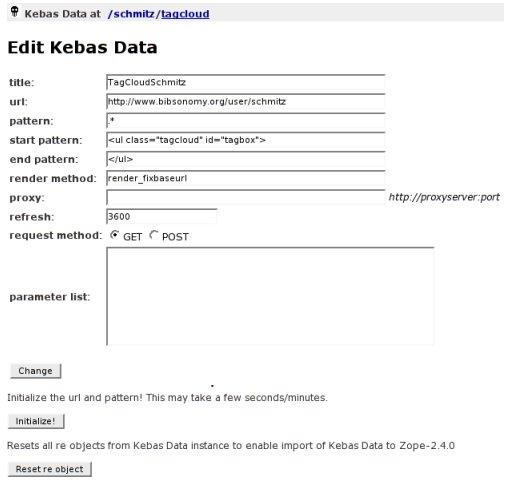
\includegraphics[width=11cm]{Bilder/tag_wolken.jpg}
 \caption{KebayData-Objekt für Tag-Wolken}
 \label{fig:kebayDataObjekt}
\end{figure}

    Es werden nun alle Tags in Ihrer Tag-Wolke angezeigt, die sich zwischen den Start- <ul ...> und den Ende- </ul> Schemata bewegen.
    \item Sie müssen jedoch die von PUMA ausgegebenen URLs überarbeiten, da diese sich auf das PUMA-Hauptverzeichnis und nicht auf Ihre Seite beziehen. Hierfür fügen Sie bitte ein \enquote{Script (Python)}-Objekt namens \textit{render\_fixbaseurl} in Zope an beliebiger Stelle oberhalb des Ordners ein, der Ihre Tag-Wolke enthält. Lassen Sie es zwei Parameter haben und folgendermaßen aussehen: 

    ul = context.match[0]\newline
    ul = ul.replace('href="/', 'href="https://puma.ub.uni-stuttgart.de/')\newline
    print ul\newline
    return printed\newline
    some code block

    \item Für die Anzeige Ihrer Tag-Wolke von \textit{DTML} aus müssen Sie diesen Befehl eingeben: 

    <ul class="tagbox">\newline
        <dtml-var tagcloud>\newline
    </ul> \newline

    \item Für die Anzeige Ihrer Tag-Wolke von einem \textit{Page Template} aus können Sie diesen Befehl benutzen: 

    <ul class=\"tagbox\">\newline
        <div tal:replace="structure here/tagcloud"/>\newline
    </ul>\newline

    \item Nutzen Sie CSS\index{CSS} zur Formatierung der Tag-Wolke nach Ihrem Geschmack. Hier sehen Sie, was wir benutzen; bitte beachten Sie, dass dies die selten vorkommenden Tags verbirgt. Sie können \textit{display: none} durch \textit{display: inline} ersetzen, um deren Anzeige zu aktivieren: 

    ul.tagbox \{ list-style: none; text-align: justify; \}\newline
    ul.tagbox li \{ display: inline; \}\newline
    ul.tagbox li a \{ display: none; text-decoration: none; color: \#e05698; font-size: 60\% \} \newline
    ul.tagbox li.tagone a \{  display: none; text-decoration: none; color: \#a3004e; font-size: 80\% \} \newline
    ul.tagbox li.tagten a \{  display: inline; text-decoration: none; color: \#830030; font-size: 100\% \} \newline
\end{enumerate}

\section{Plugins} 
\label{sec:plugins}
\subsection{OpenCms\index{OpenCms}}
\label{subsec:opencms}
Mit dem OpenCms\index{Plugins!OpenCms} Plugin bei PUMA lassen sich Publikationslisten pflegen und die bibliografischen Daten in anderen Systemen nach nutzen. Ein typischer Anwendungsfall des Plugins ist das Erstellen einer Institutspublikationsliste. Mitarbeiter und/~oder Hilfskräfte des Instituts pflegen die Publikationsdaten in PUMA ein. Die eingetragenen Publikationen können in einer Institutspublikationsliste ausgegeben und auf der Institutswebsite veröffentlicht werden. Hierbei kann zwischen mehreren Zitatiosstil ausgewählt und nach Datum in absteigender oder aufsteigender Reihenfolge sortiert werden. Das Gleiche können die Mitarbeiter ebenfalls für ihre eigenen Publikationsliste machen.
\subsubsection*{Die Umsetzung bei PUMA:}\label{sss:iplPuma}
\begin{enumerate}
\item  Anmeldung auf \url{https://puma.ub.uni-stuttgart.de.}
\item Legen Sie eine Gruppe an.
\item Mitarbeiter und/oder Hilfskräfte des Instituts tragen die Publikationen mit ihrem PUMA-Konto ein und taggen diese mit \textit{for:gruppenname}.
\item Platzieren Sie auf einer Freitextseite in OpenCms den Typ \enquote{Publikationsliste aus BibSonomy/~PUMA} aus dem Typenkatalog.
\item Füllen Sie die Eingabefelder aus.
\end{enumerate}
%\newline\newline
Eine kurze Beschreibung der Eingabefelder:\newline
%\small
\begin{longtabu}{|X|p{7cm}|}\hline
\bfseries Eingabefeld &\bfseries Beschreibung\\ \hline
Titel& 	Der Titel ist frei wählbar und erscheint auf der Seite als Überschrift, z. B. Meine Publikationen. \\ \hline
API-Benutzer­­name &	Der API-Benutzername entspricht dem von Ihnen angegebenen Benutzernamen bei PUMA. Er beginnt nach dem @-Zeichen und erscheint nach dem Login oben rechts im Benutzermenü. API steht für \enquote{Application Programming Interface} (Programmierschnittstelle, über die OpenCms und PUMA Daten austauschen).\\ \hline
API-Schlüssel &	Der API-Schlüs­sel ist ein Zahlencode, den Sie aus Ihrem Benutzermenü unter \enquote{Einstellungen} im Reiter \enquote{Einstellungen} finden und kopieren können.\\ \hline
API-Server &	Der API-Server ist bereits voreingestellt auf \url{https://puma.ub.uni-stuttgart.de/api/}\\ \hline
Quelle & Es kann aus drei möglichen Quellen ausgewählt werden: \textit{user} (Benutzerkonto), \textit{group} (Gruppenkonto) und \textit{viewable} (öffentliche Einträge im System).\\ \hline
Source-ID &	Im Feld Source-ID wird der Benutzer oder Gruppenname eingetragen. Importiert werden also die Daten aus dem jeweils angegebenen Benutzerkonto, z. B. aus dem eigenen oder den öffentlich geteilten Einträgen. Bei \textit{group} sind es dem entsprechend die Daten aus der Gruppe (z. B. schulung).\\ \hline
Tags &	Im Feld Tags (Schlagwörter) werden die Einträge eingegrenzt, die mit diesem Schlagwort vergeben sind. Eine Liste mit den eigenen Publikationen wird mit der Quelle \textit{user}, der Source-ID Benutzername und dem Tag \textit{myown} erzeugt.\\ \hline
Exclude-Tags& An dieser Stelle werden die Schlagwörter eingegeben, zu denen keine Publikationen angezeigt werden sollen.\\ \hline
Search &	Angabe eines Suchbegriffes: Komplette Volltextsuche, auch in hoch geladenen Volltexten. Ausgabe der Publikationseinträge, in denen Suchergebnisse vorkommen.\\ \hline
Anzahl der Publikationen &	Es können bis zu 1.000 Einträge angezeigt werden. Voreingestellt sind 100 Einträge.\\ \hline
Sortierfeld &	Als Sortierfeld kann \textit{none} (keine Sortierung), \textit{author} (der Autor), \textit{entrytype} (der Publikationstyp), \textit{title} (der Titel) oder \textit{year} (das Jahr) gewählt werden.\\ \hline
Sortierreihenfolge &	Definiert die auf (ascending)- oder absteigende (descending) Sortierung.\\ \hline 
Gruppierung &	Gruppierte Ausgabe mit Überschriften. Bei \textit{author} wird nach dem Alphabet (A,B,C, usw.) gegliedert. Bei \textit{entrytype} wird nach dem Publikationstyp (article, book, conference, usw.) sortiert. Mit \textit{title} werden die Publikationen nach dem Anfangsbuchstaben ihres Titels angezeigt, der erste Buchstabe erscheint als Abschnittsüberschrift. Bei \textit{year} werden die Jahreszahlen als Überschriften angezeigt.\\ \hline
Duplikatunterdrückung &	Wenn PUMA einen doppelten Publikationseintrag erkennt, wird nur einer angezeigt.\\ \hline
CSL-Stil &	Im Feld CSL-Stil (Citation Style Language) wird der Zitationsstil ausgewählt, mit dem die Publikationen angezeigt werden sollen. Falls weitere, nicht in der Liste aufgeführte Zitationsstile benötigt werden, können über die CSL-Templates bis zu 7.500 Zitationsstile ausgeben werden.\\ \hline
Zeige Zusammenfassung& 	Das Abstract, falls vorhanden, wird als Link mit ausgegeben.\\ \hline
Zeige BibTex-Code &	Der BibTex-Code kann als Link mit angezeigt werden.\\ \hline
Zeige Link & Der Link zum Volltext wird, falls vorhanden, angezeigt.\\ \hline
\label{tab:eingabefelder}
\end{longtabu}
%\normalsize
Der Inhalt der Eingabefelder für eine Mitarbeiterpublikationsliste und eine Institutspublikationsliste unterscheiden sich. Bei dem folgenden Beispiel beziehen beide Listen die Publikationen aus der Institutsgruppe in PUMA.\newline\newline
\subsubsection*{Beispiel Institutspublikationsliste:\index{Publikationslisten!Institutspublikationslisten}}\label{sss:ipl}
\begin{figure}[h!]
 \centering
 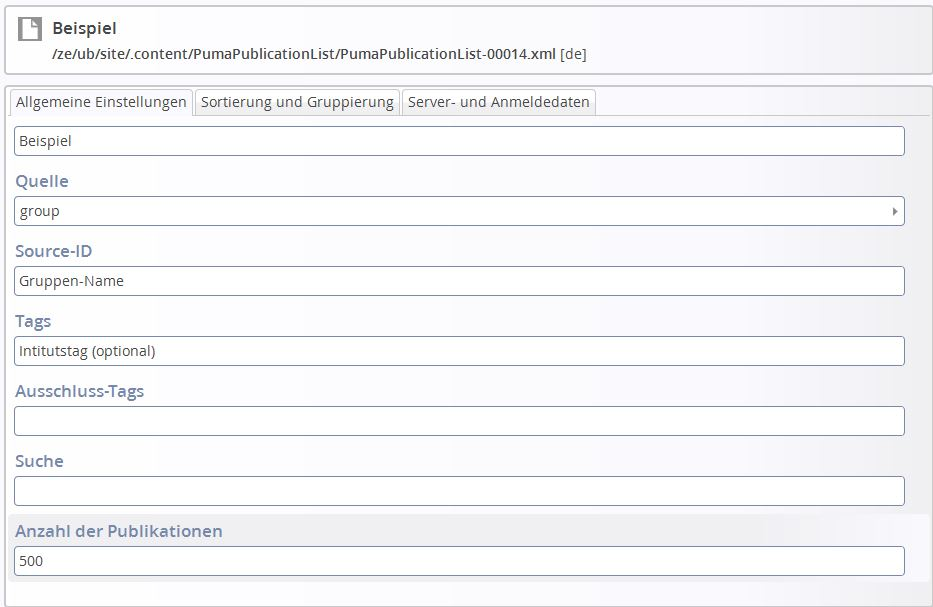
\includegraphics[width=9cm]{Bilder/Kapitel9/Institutsliste1.JPG}
 \caption{Allgemeine Einstellungen}
 \label{fig:iplAllgemeineEinstellungen}
\end{figure}\begin{figure}[h!]
 \centering
 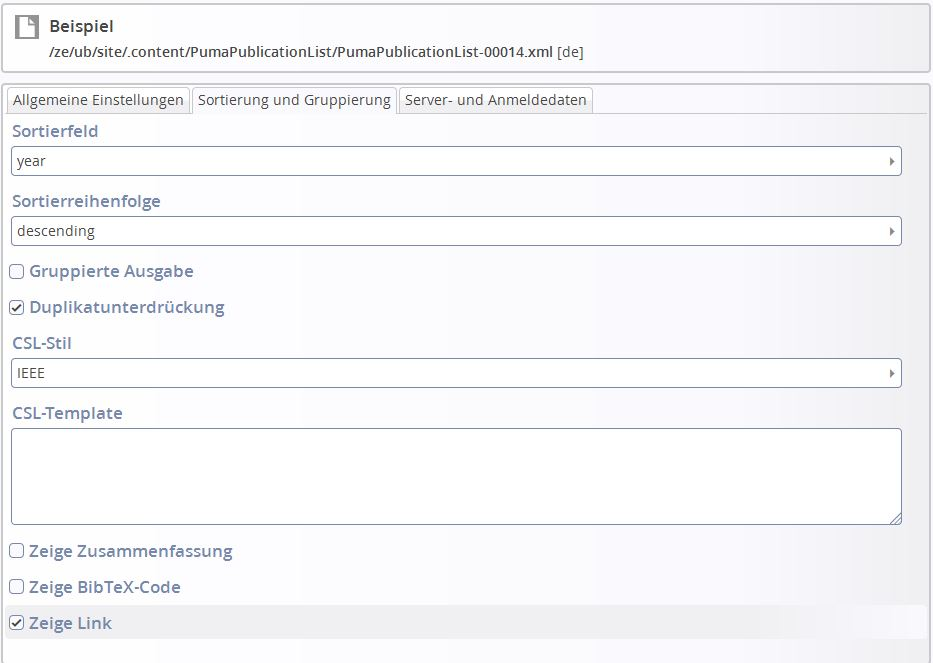
\includegraphics[width=9cm]{Bilder/Kapitel9/Institutsliste2.jpeg}
 \caption{Sortierung und Gruppierung}
 \label{fig:iplSortierungGruppierung}
\end{figure}\begin{figure}[h!]
 \centering
 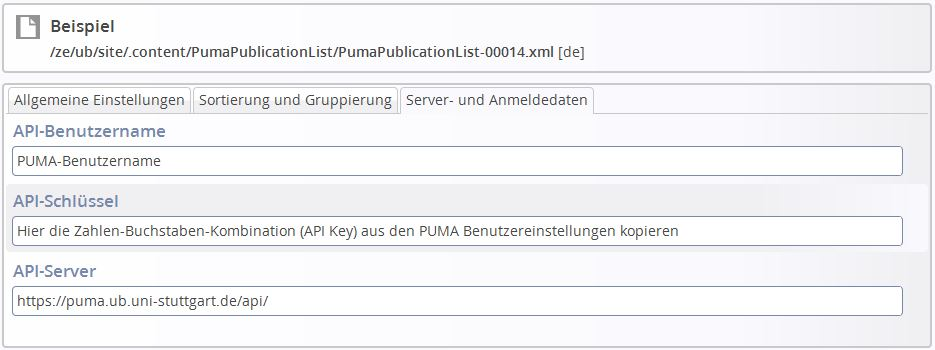
\includegraphics[width=9cm]{Bilder/Kapitel9/Institutsliste3.jpeg}
 \caption{Server- und Anmeldedaten}
 \label{fig:iplServerAnmeldedaten}
\end{figure}
\subsubsection*{Beipiel Mitarbeiterpublikationsliste}\label{sss:mpl}
\begin{figure}[h!]
 \centering
 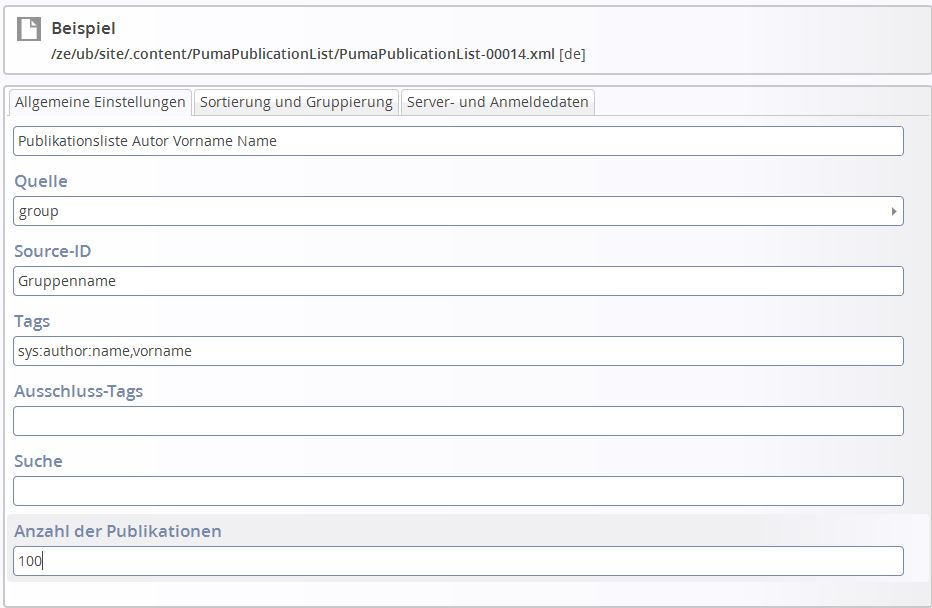
\includegraphics[width=9cm]{Bilder/Kapitel9/Mitarbeiterliste1.jpeg}
 \caption{Allgemeine Einstellungen}
 \label{fig:mplAllgemeineEinstellungen}
\end{figure}
\begin{figure}[h!]
 \centering
 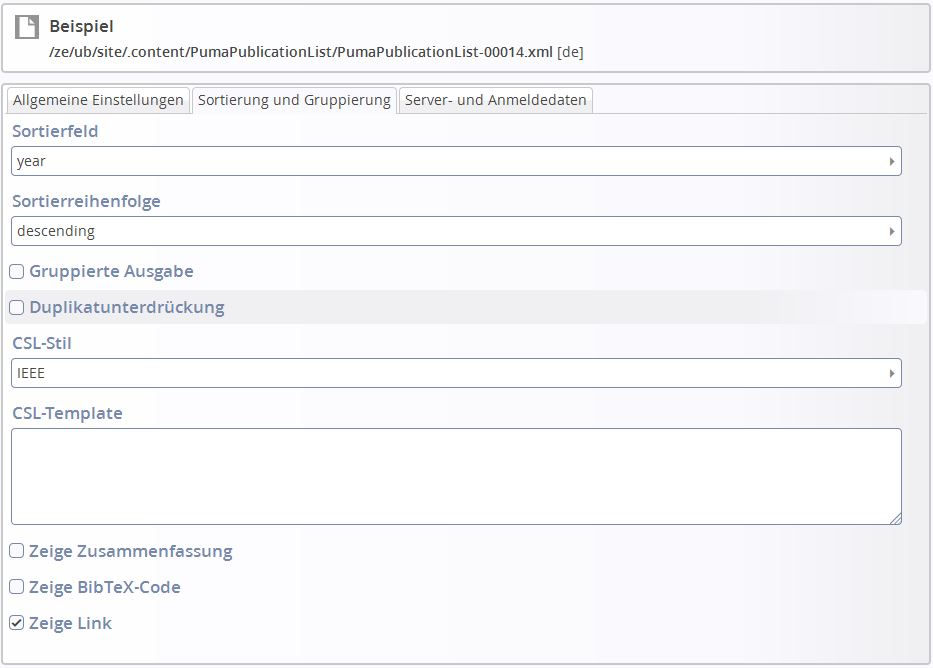
\includegraphics[width=9cm]{Bilder/Kapitel9/Mitarbeiterliste2.jpeg}
 \caption{Sortierung und Gruppierung}
 \label{fig:mplSortierungGruppierung}
\end{figure}
\begin{figure}[h!]
 \centering
 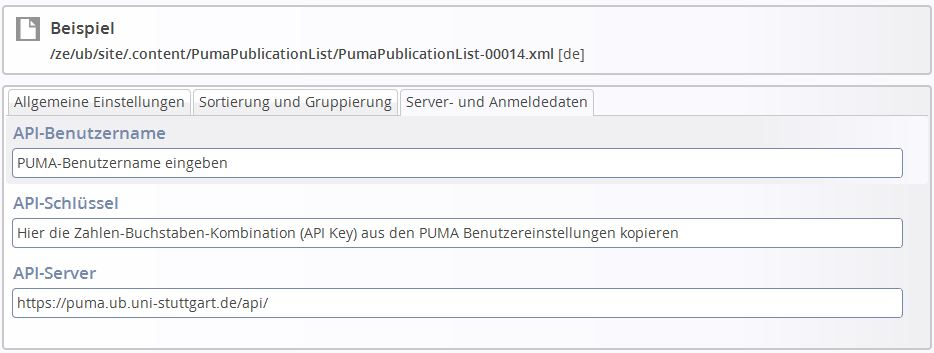
\includegraphics[width=9cm]{Bilder/Kapitel9/Mitarbeiterliste3.jpeg}
 \caption{Server- und Anmeldedaten}
 \label{fig:mplServerAnmeldedaten}
\end{figure}
Wenn die gewünschten Einstellungen veröffentlicht werden, importiert das Plugin die Literatureinträge im ausgewählten Zitationsstil auf die entsprechenden OpenCms-Seite. Veränderungen, die bei PUMA vorgenommen werden, Korrekturen oder weitere Einträge, werden automatisch auf der OpenCms-Seite aktualisiert. OpenCms-Caching-Einstellungen wirken zusätzlich, Änderungen im PUMA-System werden zeitverzögert im OpenCms sichtbar.
\subsection{Typo3\index{Typo3}}
\label{subsec:typo3}
\subsubsection*{Installation}\label{sss:installation}
Um PUMA CSL zu installieren, melden Sie sich bei Ihrer TYPO3-Instanz\index{Plugins!Typo3} als Administrator an. Gehen Sie im Extension Manager zu den Extensions Import results. Suchen Sie nach der Extension ext\_bibsonomy\_csl und importieren Sie diese.
\begin{figure}[h!]
 \centering
 \fbox{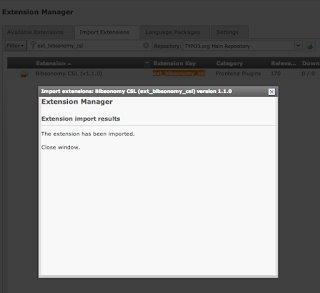
\includegraphics[width=8cm]{Bilder/Kapitel9/extension_manager.jpg}}
 \caption{Extension Manager}
 \label{fig:extensionManager}
\end{figure}
Nach erfolgreichem Import wird die Extension unter \enquote{Available Extensions} angezeigt. Klicken Sie auf das +-Symbol, um es zu aktivieren.
\begin{figure}[h!]
 \centering
 \fbox{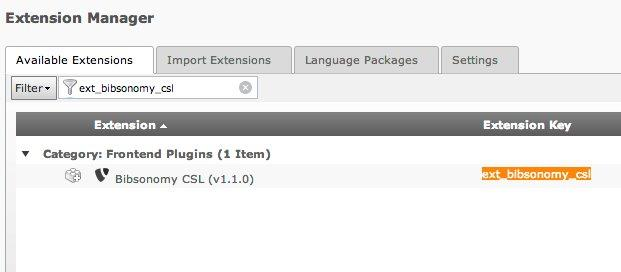
\includegraphics[width=11cm]{Bilder/Kapitel9/available_extensions.jpg}}
 \caption{Available Extensions}
 \label{fig:availableExtensions}
\end{figure}
\newline\newline
\subsubsection*{Publikationslisten hinzufügen mit dem Frontend Plugin}\label{sss:typo3Publikationslisten}
Nachdem Sie die Extension importiert und aktiviert haben, können Sie Publikationslisten erstellen. Fügen Sie dazu der Seite, auf der die Publikationsliste erscheinen soll, ein neues Plugin hinzu. Wählen Sie hierfür aus der Liste \enquote{PUMA Publication List} aus.\newline
\newline
Im Reiter \enquote{General} tragen Sie den Titel für die Publikationsliste ein.
\begin{figure}[h!]
 \centering
 \fbox{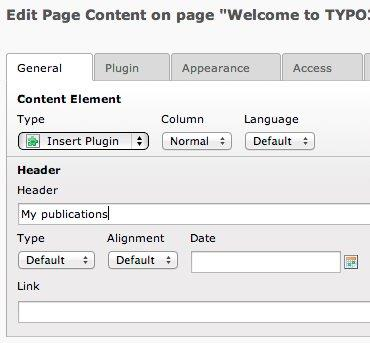
\includegraphics[width=8cm]{Bilder/Kapitel9/reiter_general.jpg}}
 \caption{Reiter General}
 \label{fig:reiterGeneral}
\end{figure}
\newline \newline
Gehen Sie auf den Reiter \enquote{Plugin} und nehmen Sie die gewünschten Einstellungen vor. Sie können zwischen \textit{user}, \textit{group} oder \textit{viewable} wählen, um den entsprechenden Inhalt aus PUMA zu definieren, den Sie in der Publikationsliste haben möchten.\newline
\newline
Beispiel: Sie möchten Ihre eigene Publikationsliste einbinden. Dazu wählen Sie zunächst unter der Rubrik \enquote{Content Source} die Option \enquote{user} aus. Tragen Sie dann den gewünschten (Ihren) Nutzernamen unter \enquote{Insert the id of user, group or viewable source} ein. Anschließend können Sie die Einträge der Publikationsliste über Tags filtern. Geben Sie hierfür die gewünschten Tags in das Feld \enquote{Select content via tags} ein. Um nur eigene Einträge anzeigen zu lassen, verwenden Sie den Systemtag \textit{myown}. Sie können zudem die Anzahl der angezeigten Publikationen begrenzen sowie mittels Freitext filtern.
\begin{figure}[h!]
 \centering
 \fbox{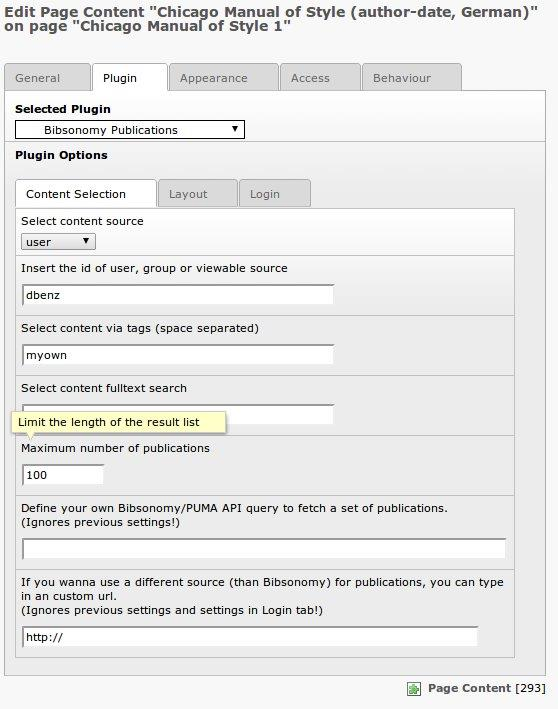
\includegraphics[width=9cm]{Bilder/Kapitel9/reiter_plugin.jpg}}
 \caption{Reiter Plugin}
 \label{fig:reiterPlugin}
\end{figure}

\begin{mdframed}[style=mdfexample1,frametitle={ACHTUNG},backgroundcolor=gray!40]Bitte beachten Sie, dass die Extension Ihre gesamte Publikationsliste darstellt, wie Sie sie in PUMA sehen \textbf{(auch private Publikationen)}. Wenn Sie z.B. an eine Publikation ein Dokument angehängt haben, dann wird dieses auch in der Publikationsliste angezeigt. Dadurch können für Sie \textbf{urheberrechtliche Konsequenzen} entstehen. Wir empfehlen Ihnen daher für die Nutzung einen zusätzlichen Account anzulegen, mit dem Sie in PUMA nur die TYPO3-Publikationen verwalten.
\end{mdframed} 
In der Rubrik \enquote{Layout} können Sie die Gestaltung der Publikationsliste anpassen. Dies geschieht durch Citation Style Language (CSL\index{CSL}), das ist eine frei verfügbare XML-basierte Auszeichnungssprache. Eine große Liste an frei verfügbaren CSL-Vorlagen finden Sie hier: \url{http://www.zotero.org/styles/}.
\begin{figure}[h!]
 \centering
 \fbox{
\includegraphics[width=7cm]{Bilder/Kapitel9/csl_typo.jpg}}
 \caption{Citation Style Language(CSL)}
 \label{fig:csl}
\end{figure}

In der letzten Rubrik \enquote{Login} müssen Sie Ihre PUMA API-Daten\index{API} hinterlegen. Nur so kann sich die TYPO3 Extension bei PUMA anmelden und Ihre Daten abrufen. Ihre API-Daten finden Sie, wenn Sie über das Personensymbol in die Einstellungen gehen und im Reiter \enquote{Einstellungen} nach unten scrollen. 
\subsubsection*{Tag-Wolken hinzufügen mit dem Frontend Plugin}\label{sss:typo3Tagwolken}
Sie können Ihren Webseiten nicht nur Publikationslisten hinzufügen, sondern auch Ihre PUMA  Tag-Wolke(Tagcloud). Fügen Sie dazu der Seite, auf der die Tag-Wolke\index{Tag!Wolke} erscheinen soll, ein neues Plugin hinzu. Wählen Sie aus der Liste \enquote{Bibsonomy Tag Cloud}.\newline \newline 
Wie bei \enquote{Publikationsliste hinzufügen} können Sie auch hier zwischen verschiedenen Modi wählen.\newline \newline 
\subsubsection*{CSL Styles mit dem Backend-Module verwalten}\label{typo3CslBackend}
\newline
TYPO3-Extensions werden klassisch in zwei Module unterteilt, dem Frontend- und Backend-Module. Die Frontend-Module \enquote{Publikationsliste hinzufügen} und \enquote{Tag-Wolke hinzufügen} wurden bereits erklärt. In diesem Abschnitt soll es um das Backend-Modul gehen, mit dem Sie die CSL-Stylesheets verändern können.\newline \newline
Bereits mit der Extension-Installation werden Ihnen eine Reihe von CSL-Stylesheets ausgeliefert. Um weitere Stylesheets hinzuzufügen, erstellen Sie einen neuen Ordner im Seitenbaum und nennen diesen \textit{CSL Styles}. Wählen Sie anschließend diesen Ordner aus. Klicken Sie auf \enquote{Neu} und wählen \enquote{Add a custom style}.\newline \newline
Um ein neue Stylesheets hinzuzufügen gibt es drei unterschiedliche Möglichkeiten:
\begin{enumerate}
\item Geben Sie den XML-Quellcode direkt in das Textfeld ein und klicken Sie anschließend auf \enquote{Save}.
\item Geben Sie in das Textfeld die URL des CSL-Stylesheets ein und klicken Sie auf \enquote{Import}.
\item Laden Sie ein CSL-Stylesheet von Ihrem Computer hoch und klicken Sie auf anschließend auf \enquote{Upload}. 
\end{enumerate}
\begin{figure}[h!]
 \centering
 \fbox{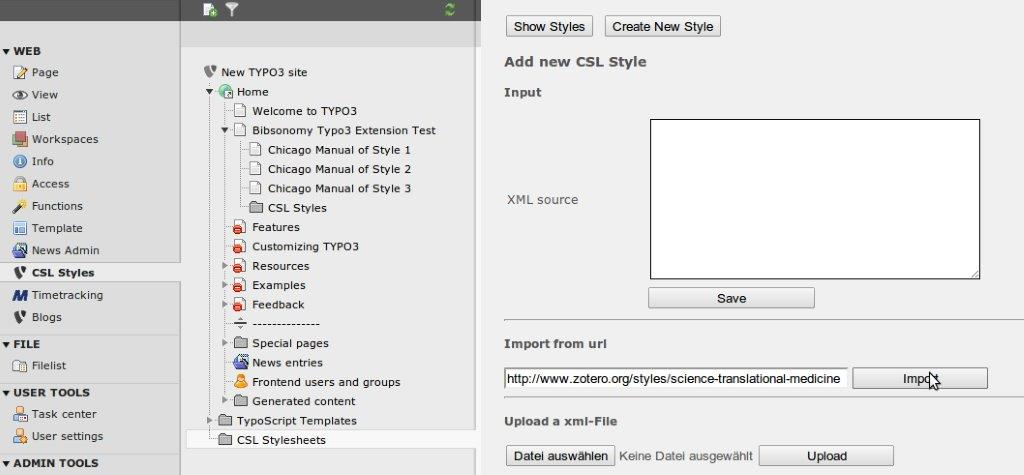
\includegraphics[width=11cm]{Bilder/Kapitel9/stylesheets.jpg}}
 \caption{Neue Stylesheets hinzuzufügen}
 \label{fig:neueStylesheets}
\end{figure}
Um eine Vorschau zu erhalten, klicken Sie auf \enquote{Show Styles}.\newline
Um eine CSL-Stylesheet zu löschen klicken Sie wie gewohnt auf das Mülleimersymbol in Typo3. 
\begin{figure}[h!]
 \centering
 \fbox{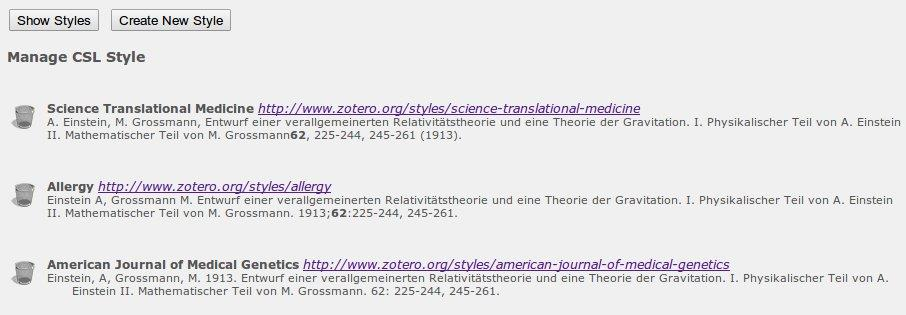
\includegraphics[width=11cm]{Bilder/Kapitel9/csl_stylesheet.jpg}}
 \caption{CSL-Stylesheet löschen}
 \label{fig:cslLoeschen}
\end{figure}
\subsection{WordPress\index{WordPress}}
\label{subsec:wordpress}
Das WordPress-Plugin\index{Plugins!WordPress} ermöglicht Ihnen verschiedene PUMA-Funktionen für Ihren eigene WordPress-Blog zu nutzen.\newline\newline
\textbf{Die Funktionen:}
\begin{enumerate}
   \item Fügen Sie Publikationslisten in einen Artikel ein, indem Sie die Meta-Box-Integration nutzen
    \item Sie können alternativ die WordPress-Shortcodes nutzen
    \item Wählen Sie Ihre Publikationen aus verschiedenen Inhaltstypen aus (z.~B. user/group/viewable)
    \item Filtern Sie die Ergebnisse mit Tags oder einer Volltextsuche
    \item Wählen Sie Ihren bevorzugten Zitierstil (Citation Style Language (CSL))\footnote{\url{ http://citationstyles.org/}}  aus einer Liste aus vorinstallierten Stilen aus
    \item Sie können Ihren eigenen Zitierstil mit Hilfe der CSL\index{CSL} nutzen oder erstellen, um Ihre Literaturliste anzeigen zu lassen
    \item Sie können das Layout Ihrer Liste mit CSS bearbeiten
    \item Speichern Sie Ihre API-Einstellungen (z.B. API-Nutzer, API-Key) auf einer separaten Optionsseite für Administratoren
    \item Fügen Sie Ihrem Blog Tagwolken aus PUMA hinzu und wählen Sie zwischen drei verschiedenen Layouts aus
    \item Stellen Sie Dokumente, die an Publikationen angehängt worden sind, zum Download bereit
\end{enumerate} 
Um Publikationslisten basierend auf der Citation Style Language zu erstellen wird das WordPress-Plugin benötigt. Unter folgender Website kann das Plugin installiert werden: \url{https://wordpress.org/plugins/bibsonomy-csl/}. Eine Anleitung zur Installation finden Sie im BibSonomy Blog \footnote{\url{http://blog.bibsonomy.org/2012/12/feature-of-week-add-publication-lists.html}}
%\subsection{Ilias}
%\label{subsec:ilias}
%\subsection{Moodle}
%\label{subsec:moodle}
%Das PUMA/BibSonomy Module (PBM) ist das PUMA/BibSonomy Plugin für Moodle. Es ermöglicht das Veröffentlichen von Publikationslisten aus PUMA heraus in einen Moodlekurs. Der Zitationsstil, in welchem die Publikationen in Moodle angezeigt werden sollen, kann mit Hilfe des CSL\footnote{\url{http://citationstyles.org/}} festgelegt werden.\newline\newline
%\textbf{ Der Administrator}\newline
%Die folgenden Schritte sind wichtig für die Installation des PBM Plugins: 
%\begin{enumerate}
	%\item Laden Sie sich das Plugin als \*.zip Datei herunter. Wählen Sie auf der Seite von Moodle (\url{https://moodle.org/plugins/view.php?plugin=mod_pbm} ) den Reiter \enquote{Version} aus und klicken auf Download.
	%\item Entpacken Sie die \*.zip Datei im  richtigen Ordner (z.B. /var/www/moodle/mod/pbm)
	%\item Gehen Sie auf die Moodle Webseite und loggen Sie sich als Administrator ein. Gehen Sie unter Einstellungen auf \enquote{Website-Administration} wählen Sie \enquote{Plugins} aus. Klicken Sie anschließend auf\enquote{Plugin-Übersicht}.
	%\item Klicken Sie oben auf der Überblickseite der Plugins auf den Button \enquote{Alle verfügbaren Updates überprüfen}.
	%\item Moodle informiert Sie darüber, dass das Database Update durchgeführt wurde. Bestätigen Sie dies.     
	%\item Sie werden nach einer voreingestellten Serveradresse gefragt, nach Ihren OAuth Consumer-Daten und Ihrer Wahl des Zitationsstils.      
%\end{enumerate}   
%Für die Konfiguration füllen Sie bitte folgende Felder aus:\newline\newline   
%\textbf{Default PBM Server:} Fügen Sie in dieses Feld die URL von PUMA Stuttgart ein (\url{https://puma.ub.uni-stuttgart.de/}). Diese wird ab sofort als Standard verwendet, wenn ein PBM zum Moodle-Kurs hinzugefügt wird.\newline\newline
%\textbf{Comsumer-Key/Consumer-Secret(Optional):}Der Administrator eines Moodle-Kurses kann in den lokalen Administrations-Einstellungen eine OAuth -Nutzer- Bestätigung erstellen. Diese wird dazu verwendet, um die Accounts der Nutzer über die OAuth Authentifizierung mit PUMA zu verknüpfen. \newline\newline
%\textbf{Available CSL files:}Hier können Sie zwischen unterschiedlichen Zitationsstilen auswählen. Weitere Informationen über Zitationsstile gibt es unter \url{http://citationstyles.org/}.
%\newline\newline
%\textbf{Nutzer}\newline
\section{Bitbucket\index{Bitbucket}}
\label{sec:bitbucket}
Bitbucket ist ein auf Git basierendes Versionskontrollsystem, das die Zusammenarbeit mit Teams erleichtert.  
\newline
Bei Problemen oder Fehlern können die Nutzer diese in Bitbucket melden und die Entwickler kümmern sich sofort darum. Hier benötigen die Nutzer ein eigens Bitbucket-Nutzerkonto. Mit diesem melden Sie sich bei Bitbucket an und gehen auf die Bibsonomy/~Puma-Seite\footnote{\url{https://bitbucket.org/bibsonomy/puma}}. Unter dem Reiter \enquote{Issues} können neue Problemmeldungen verfasst werden.
